\chapter{CellTAN Development}

\section{Statistical tests for measuring association} \label{ap1:stats}

\subsection{Pearson's chi squared test} \label{ap1:pearsonschi}

\begin{equation}
    \chi^2 = \sum_{i=1}^{k} \frac{(O_i - E_i)^2}{E_i}
\end{equation}
    
where:
\begin{align*}
\chi^2 & : \text{Chi-squared statistic} \\
O_i & : \text{Observed frequency for category } i \\
E_i & : \text{Expected frequency for category } i \\
k & : \text{Number of categories or cells in the data}
\end{align*}


\subsection{Fischer's exact test} \label{ap1:fischer}

\begin{equation}
    p = \frac{{\binom{a}{x} \binom{b}{y}}}{{\binom{N}{n}}}
\end{equation}

where:
\begin{align*}
    p & : \text{p-value of the test} \\
    a & : \text{Number of successes in group A} \\
    b & : \text{Number of successes in group B} \\
    x & : \text{Number of successes of interest in group A} \\
    y & : \text{Number of successes of interest in group B} \\
    N & : \text{Total number of observations} \\
    n & : \text{Number of observations in group A}
\end{align*}


\subsection{Odds ratio} \label{ap1:oddsratio}

\begin{equation}
OR = \frac{{a \cdot d}}{{b \cdot c}}
\end{equation}

where:
\begin{align*}
OR & : \text{Odds ratio} \\
a & : \text{Number of successes in group A} \\
b & : \text{Number of failures in group A} \\
c & : \text{Number of successes in group B} \\
d & : \text{Number of failures in group B}
\end{align*}

\subsection{Phi coefficient} \label{ap1:phi}

\begin{equation}
\phi = \sqrt{\frac{\chi^2}{N}}
\end{equation}

where:
\begin{align*}
\phi & : \text{Phi coefficient} \\
\chi^2 & : \text{Chi-squared statistic} \\
N & : \text{Total number of observations}
\end{align*}

\subsection{Contingency coefficient C} \label{ap1:contingencyc}

\begin{equation}
C = \sqrt{\frac{\chi^2}{N + \chi^2}}
\end{equation}

where:
\begin{align*}
C & : \text{Contigency coefficient} \\
\chi^2 & : \text{Chi-squared statistic} \\
N & : \text{Total number of observations}
\end{align*}


\subsection{Theil's U} \label{ap1:theilsu}

\begin{equation}
U(x|y) = \frac{H(x) - H(x|y)}{H(x)}
\end{equation}

Entropy of variable x:
\begin{equation}
H(x) = -\sum_{i=1}^{n} p(x_i) \log(p(x_i))
\end{equation}

Conditional entropy of variable x given variable y:
\begin{equation}
H(x|y) = -\sum_{i=1}^{n} \sum_{j=1}^{m} p(x_i, y_j) \log\left(\frac{p(x_i, y_j)}{p(y_j)}\right)
\end{equation}


\section{Technology stack} \label{ap1:techstack}

\begin{figure}[h!]
    \centering
    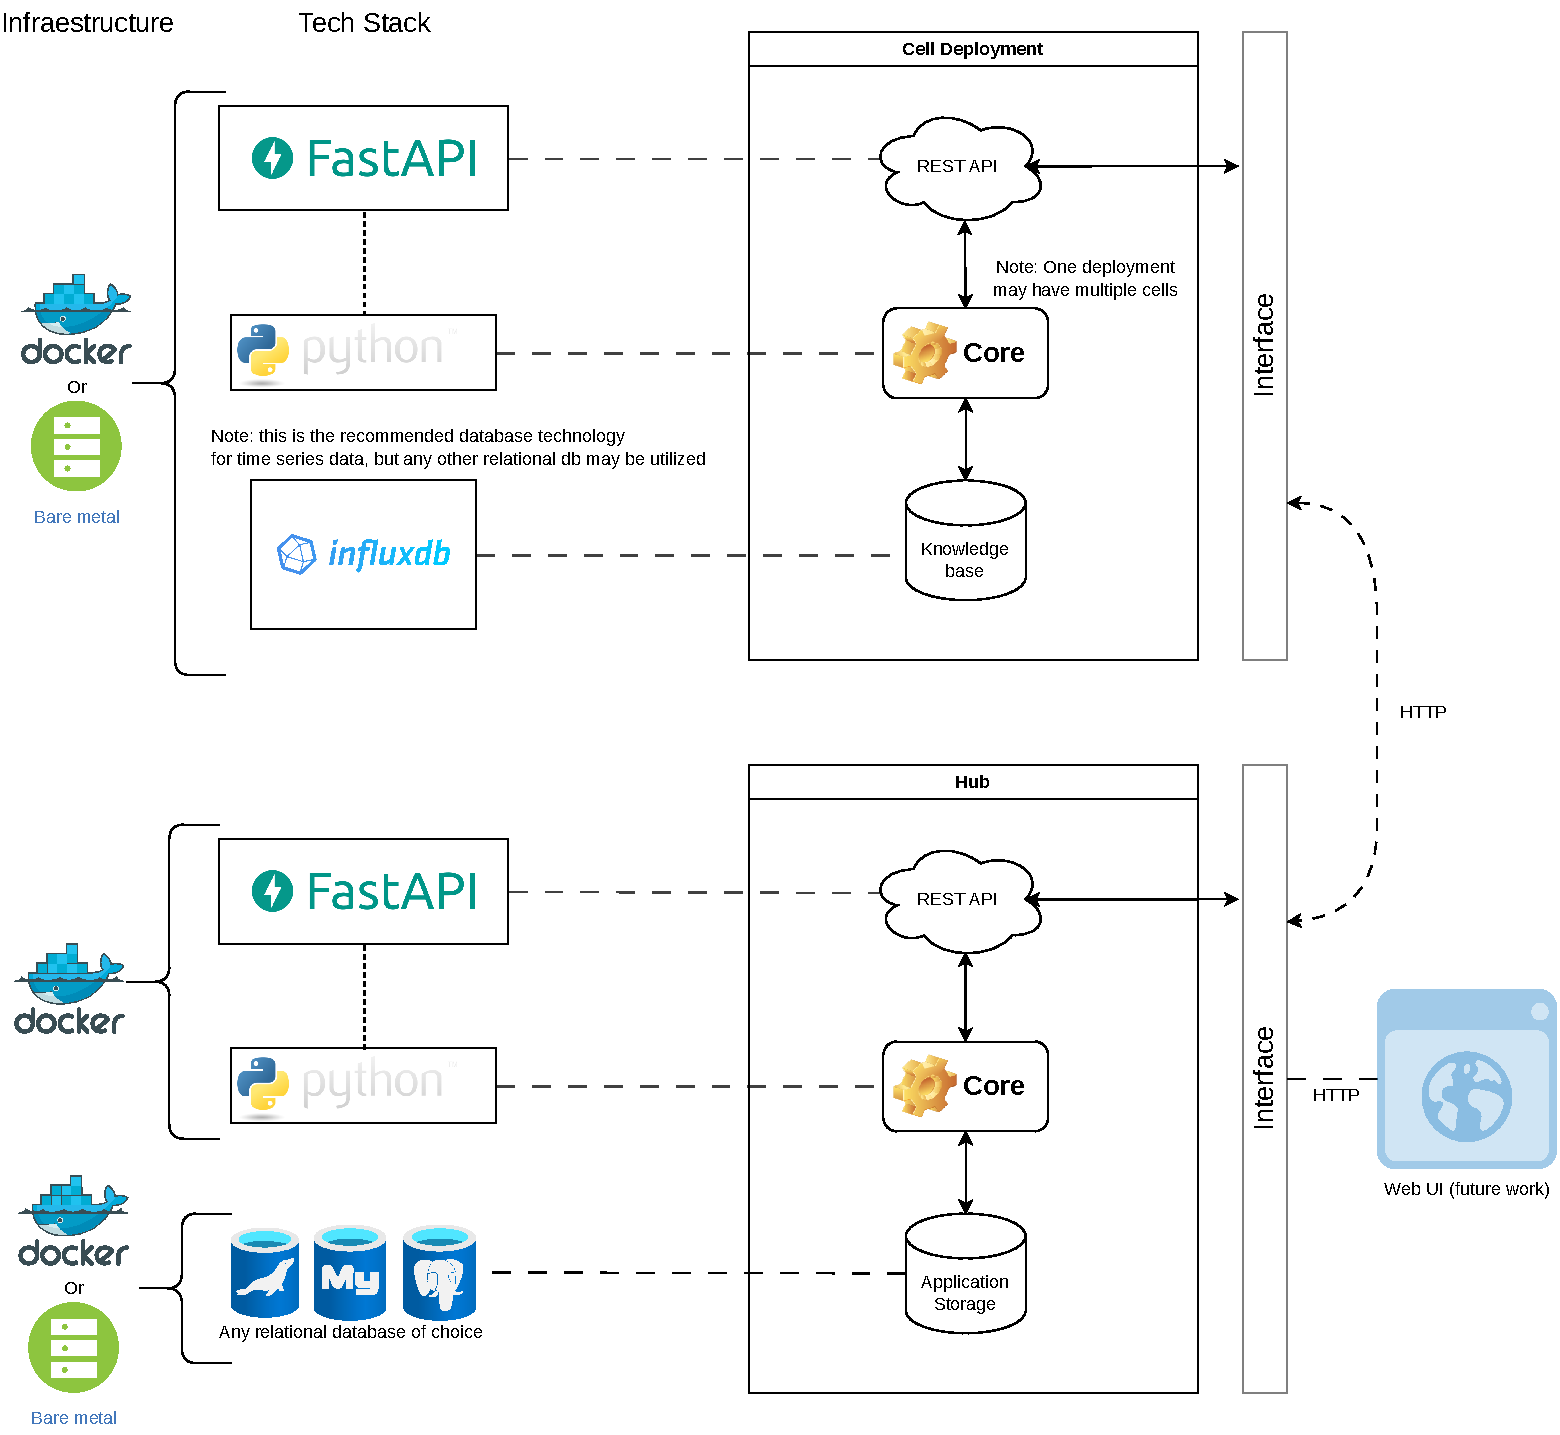
\includegraphics[width=\linewidth]{figures/appendix/a_development/techstack.pdf}
    \caption{Technology stack of the Cell and Hub of CellTAN.}
    \label{fig:techstack}
\end{figure}


\section{Cell configuration} \label{ap1:config}
 
The idea for configuring cells before deployment is to have a text file with every necessary parameter. As mentioned in \ref{subsec:cellconfig}, I chose the YAML format for laying out cell information, coupled with a Pydantic \cite{pydantic} model that mirrors the file entries with attributes of the correct types in Python.

The following fields define input variables:
\begin{itemize}
    \item id: Variable identifier, e.g. "dc\_voltage".
    \item uncertainty: The percentage uncertainty of the variable relative to its range (maximum value - minimum value).
    \item minimum: The minimum possible value for the variable.
    \item maximum: The maximum possible value for the variable.
    \item time\_decay: The time it takes for the variable to reach full uncertainty.
\end{itemize}

The cell has the following thresholds:

\begin{itemize}
	\item min\_knowledge\_for\_raising\_new\_experience: Minimum time window that the knowledge base needs to have for the cell to flag new experiences.

    \item min\_trust\_for\_filtering: Minimum value required of the instantaneous trust measurement with a neighbor for the cell to use its activations for output computation.
	
    \item min\_trust\_for\_uncomformity: The trust threshold used to detect extrinsic unconformity.
	
    \item goal\_neighbors\_frac\_for\_activations: Goal fraction of neighbors with recent activations, used for retrying the process of activation fetching.
	
    \item rolling\_timestamp\_offset: The time offset between the present and time associated with the inputs' values. Allows using cells with forecast values.
	
    \item trust\_comparison\_bins: List of time windows for which the cell compares historical trust measures for neighbors' and variables' trust. 
	
    \item max\_knowledge\_time\_diff: Maximum time difference between two pieces of knowledge to consider or discard such. For example, if neighbors' activations were calculated longer ago than this value, the cell does not consider them.
	
    \item min\_loop\_sleep: Minimum time the cell must remain in stand-by mode between each cycle. It avoids computational overload if overwhelmed with high-frequency inputs update.
	
    \item max\_loop\_sleep: Maximum time the cell may remain in standby mode. This ensures that if no inputs arrive, it will periodically update its attributes to reflect the increased uncertainty of its inputs (due to the time decay process).
\end{itemize}
